\documentclass[aspectratio=169,11pt]{beamer}
\usetheme{metropolis}
\usepackage{tikz}
\usetikzlibrary{arrows.meta,positioning,calc}
\usepackage{booktabs}
\usepackage{xcolor}
\usepackage{amsmath}
\usepackage{hyperref}
\usepackage{array}
\newcolumntype{L}[1]{>{\raggedright\arraybackslash}p{#1}}
\hyphenpenalty=10000
\exhyphenpenalty=10000

% === Color palette ===
\definecolor{report}{HTML}{3498DB}
\definecolor{state}{HTML}{9B59B6}
\definecolor{bias}{HTML}{E67E22}
\definecolor{neutral}{HTML}{95A5A6}
\definecolor{pass}{HTML}{27AE60}
\definecolor{fail}{HTML}{E74C3C}
\tikzset{
  box/.style={draw=#1,thick,rounded corners,fill=#1!10,minimum width=3.2cm,minimum height=0.9cm,font=\small,align=center},
  boxL/.style={draw=#1,thick,rounded corners,fill=#1!10,minimum width=5.2cm,minimum height=1.2cm,font=\small,align=center},
  boxS/.style={draw=#1,thick,rounded corners,fill=#1!10,minimum width=2.8cm,minimum height=0.9cm,font=\footnotesize,align=center},
  panel/.style={draw=#1,thick,rounded corners,fill=#1!8},
}
\hypersetup{colorlinks=true,linkcolor=.,urlcolor=report}

% Metropolis sizes its title page to \paperheight, which overfills a plain frame by ~16pt.
\makeatletter
\setbeamertemplate{title page}{
  \begin{minipage}[b][\dimexpr\paperheight-16pt\relax]{\textwidth}
    \vfill%
    \ifx\inserttitle\@empty\else\usebeamertemplate*{title}\fi
    \ifx\insertsubtitle\@empty\else\usebeamertemplate*{subtitle}\fi
    \usebeamertemplate*{title separator}
    \ifx\beamer@shortauthor\@empty\else\usebeamertemplate*{author}\fi
    \ifx\insertdate\@empty\else\usebeamertemplate*{date}\fi
    \ifx\insertinstitute\@empty\else\usebeamertemplate*{institute}\fi
    \vfill
    \vspace*{1mm}
  \end{minipage}
}
\makeatother

\title{Metrology and Robustness}
\subtitle{The vocabulary of measurement, and agreement as evidence}
\author{Measuring AI Self-Reports}
\date{}
\institute{}

\newcommand{\partslide}[2]{%
\begin{frame}[plain,label=#1]
\vfill
\begin{center}
  \setlength{\fboxrule}{2.5pt}%
  \fcolorbox{black}{white}{\parbox{0.65\textwidth}{\centering\vspace{0.8em}
    {\Large\bfseries #2}
  \vspace{0.8em}}}
\end{center}
\vfill
\end{frame}}

\begin{document}

\maketitle

%% --- Overview ---
\begin{frame}{Overview}\footnotesize
\begin{columns}[T]
\begin{column}{0.48\textwidth}
\hyperlink{part1}{\textbf{Part 1: One measurement, term by term}}\\[0.15em]
{\scriptsize%
\quad\hyperlink{picture}{1.~Metrology in one picture}\\%
\quad\hyperlink{measurand}{2.~Measurand}\\%
\quad\hyperlink{gaps}{3.~Measurand and realized quantity}\\%
\quad\hyperlink{indication}{4.~Indication, model and result}\\%
\quad\hyperlink{calibration}{5.~Calibration and traceability}\\%
\quad\hyperlink{uncertainty}{6.~Uncertainty and its floor}\\%
\quad\hyperlink{sources}{7.~Sources of uncertainty}\\%
\quad\hyperlink{compare}{8.~Comparability and compatibility}\\%
\quad\hyperlink{validation}{9.~Validation for an intended use}%
}\vspace{0.3em}

\hyperlink{part2}{\textbf{Part 2: The introspection experiment}}\\[0.15em]
{\scriptsize%
\quad\hyperlink{injection}{10.~Concept injection}\\%
\quad\hyperlink{mapping}{11.~The experiment in the vocabulary}\\%
\quad\hyperlink{twosenses}{12.~Two senses of calibration}\\%
\quad\hyperlink{llmunc}{13.~Uncertainty in an injection experiment}\\%
\quad\hyperlink{limitsmet}{14.~Where the analogy stops: metrology}%
}
\end{column}
\begin{column}{0.48\textwidth}
\hyperlink{part3}{\textbf{Part 3: Robustness and convergence}}\\[0.15em]
{\scriptsize%
\quad\hyperlink{wimsatt}{15.~Robustness analysis}\\%
\quad\hyperlink{illusory}{16.~Illusory robustness}\\%
\quad\hyperlink{cf}{17.~Independence of methods}\\%
\quad\hyperlink{perrin}{18.~Perrin's convergence and Hudson's reading}\\%
\quad\hyperlink{islands}{19.~Coherence and islands}%
}\vspace{0.3em}

\hyperlink{part4}{\textbf{Part 4: Robustness in AI introspection}}\\[0.15em]
{\scriptsize%
\quad\hyperlink{shared}{20.~A report and a probe on the same activations}\\%
\quad\hyperlink{structure}{21.~Convergence, calibration and islands}\\%
\quad\hyperlink{limitsrob}{22.~Where the analogy stops: robustness}\\%
\quad\hyperlink{summary}{23.~Summary}\\%
\quad\hyperlink{reading}{24.~Reading}%
}
\end{column}
\end{columns}
\end{frame}

%% ============================================================
\partslide{part1}{Part 1\\[0.5em]{\large\mdseries One measurement, term by term}}
%% ============================================================

\begin{frame}[label=picture]{Metrology in one picture}
Metrology is the science of measurement. The
\href{https://www.bipm.org/documents/20126/2071204/JCGM_200_2012.pdf}{International Vocabulary of Metrology (VIM)} defines its terms, and the
\href{https://www.bipm.org/documents/20126/2071204/JCGM_100_2008_E.pdf}{Guide to the Expression of Uncertainty in Measurement (GUM)} sets the rules for uncertainty.

\vspace{0.5em}
\begin{center}
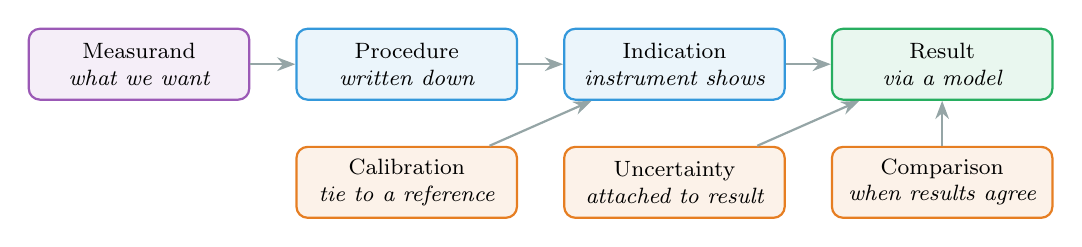
\begin{tikzpicture}
  \node[boxS=state] (m) at (0,0) {Measurand\\{\footnotesize\itshape what we want}};
  \node[boxS=report] (p) at (3.4,0) {Procedure\\{\footnotesize\itshape written down}};
  \node[boxS=report] (i) at (6.8,0) {Indication\\{\footnotesize\itshape instrument shows}};
  \node[boxS=pass] (r) at (10.2,0) {Result\\{\footnotesize\itshape via a model}};
  \draw[-{Stealth},thick,neutral] (m) -- (p);
  \draw[-{Stealth},thick,neutral] (p) -- (i);
  \draw[-{Stealth},thick,neutral] (i) -- (r);
  \node[boxS=bias] (c) at (3.4,-1.5) {Calibration\\{\footnotesize\itshape tie to a reference}};
  \node[boxS=bias] (u) at (6.8,-1.5) {Uncertainty\\{\footnotesize\itshape attached to result}};
  \node[boxS=bias] (k) at (10.2,-1.5) {Comparison\\{\footnotesize\itshape when results agree}};
  \draw[-{Stealth},thick,neutral] (c) -- (i);
  \draw[-{Stealth},thick,neutral] (u) -- (r);
  \draw[-{Stealth},thick,neutral] (k) -- (r);
\end{tikzpicture}
\end{center}

\vspace{0.4em}
{\small The measurement card on this site takes its stages from these texts. The GUM adds that a result is complete only with a statement of its uncertainty (3.1.2).}
\end{frame}

\begin{frame}[label=measurand]{Measurand}
The \textbf{\textcolor{state}{measurand}} is the quantity you intend to measure (VIM~2.3). You specify it by description: the kind of quantity, and the state of the thing that carries it.

\vspace{0.4em}
\begin{center}
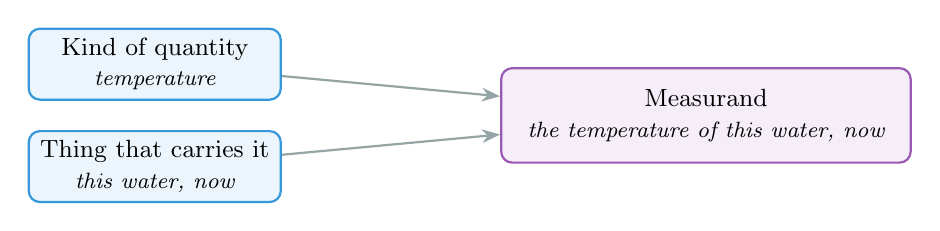
\begin{tikzpicture}
  \node[box=report] (k) at (0,0.65) {Kind of quantity\\{\footnotesize\itshape temperature}};
  \node[box=report] (s) at (0,-0.65) {Thing that carries it\\{\footnotesize\itshape this water, now}};
  \node[boxL=state] (m) at (7,0) {Measurand\\{\footnotesize\itshape the temperature of this water, now}};
  \draw[-{Stealth},thick,neutral] (k) -- (m);
  \draw[-{Stealth},thick,neutral] (s) -- (m);
\end{tikzpicture}
\end{center}

\vspace{0.4em}
How much detail is enough? The GUM's answer (3.1.3): enough that, for the purposes at hand, the measurand has a \textbf{unique value}.

\vspace{0.3em}
{\small A thermometer is the running example for the rest of this part.}
\end{frame}

\begin{frame}[label=gaps]{Measurand and realized quantity}
Three gaps can open between the measurand and what actually gets measured:

\vspace{0.5em}
\begin{center}
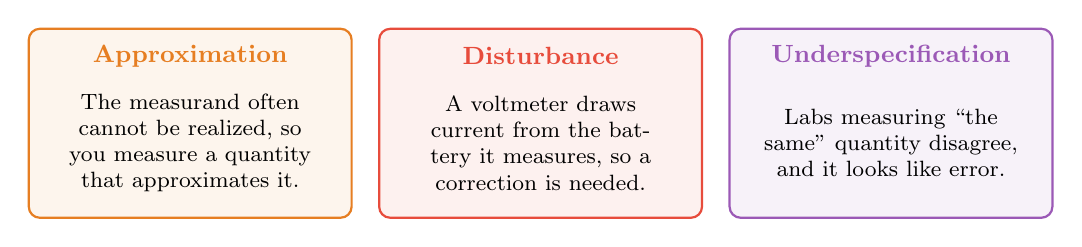
\begin{tikzpicture}
  \draw[panel=bias] (0,0) rectangle (4.1,2.4);
  \node[font=\small\bfseries,text=bias] at (2.05,2.05) {Approximation};
  \node[font=\footnotesize,align=center,text width=3.7cm] at (2.05,0.95) {The measurand often cannot be realized, so you measure a quantity that approximates it.};
  \draw[panel=fail] (4.45,0) rectangle (8.55,2.4);
  \node[font=\small\bfseries,text=fail] at (6.5,2.05) {Disturbance};
  \node[font=\footnotesize,align=center,text width=3.7cm] at (6.5,0.95) {A voltmeter draws current from the battery it measures, so a correction is needed.};
  \draw[panel=state] (8.9,0) rectangle (13.0,2.4);
  \node[font=\small\bfseries,text=state] at (10.95,2.05) {Underspecification};
  \node[font=\footnotesize,align=center,text width=3.7cm] at (10.95,0.95) {Labs measuring ``the same'' quantity disagree, and it looks like error.};
\end{tikzpicture}
\end{center}

\vspace{0.5em}
{\small Sources: GUM~D.2.1, VIM~2.3 (Note~3), GUM~D.3.4. The third gap returns in Part~2: a vague measurand produces disagreement between labs that looks like instrument error.}
\end{frame}

\begin{frame}[label=indication]{Indication, model and result}
The \textbf{procedure} describes the measurement in detail (VIM~2.6). Running it gives an \textbf{\textcolor{report}{indication}}: the value the instrument provides (VIM~4.1).

\vspace{0.3em}
\begin{center}
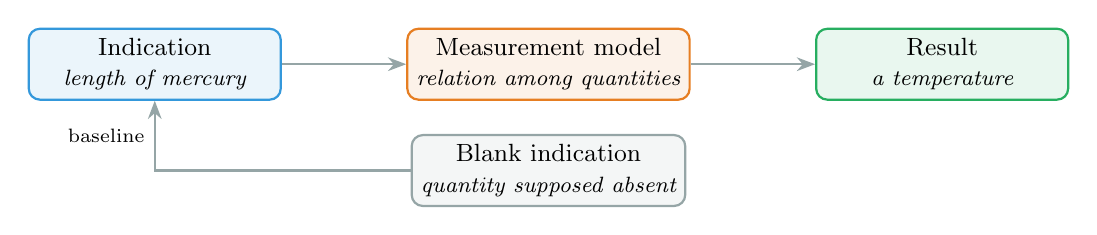
\begin{tikzpicture}
  \node[box=report] (i) at (0,0) {Indication\\{\footnotesize\itshape length of mercury}};
  \node[box=bias] (mm) at (5,0) {Measurement model\\{\footnotesize\itshape relation among quantities}};
  \node[box=pass] (r) at (10,0) {Result\\{\footnotesize\itshape a temperature}};
  \draw[-{Stealth},thick,neutral] (i) -- (mm);
  \draw[-{Stealth},thick,neutral] (mm) -- (r);
  \node[box=neutral] (b) at (5,-1.35) {Blank indication\\{\footnotesize\itshape quantity supposed absent}};
  \draw[-{Stealth},thick,neutral] (b.west) -| node[pos=0.75,left,font=\scriptsize,text=black]{baseline} (i.south);
\end{tikzpicture}
\end{center}

\vspace{0.2em}
{\small The indication belongs to the instrument; the result is a claim about the measurand (VIM~2.9), and the two need not be the same kind of quantity. The \textbf{blank indication} (VIM~4.2) is the reading where the quantity is supposed to be absent. It finds the instrument's baseline.}
\end{frame}

\begin{frame}[label=calibration]{Calibration and traceability}
\textbf{\textcolor{bias}{Calibration}} has two steps (VIM~2.39):

\begin{center}
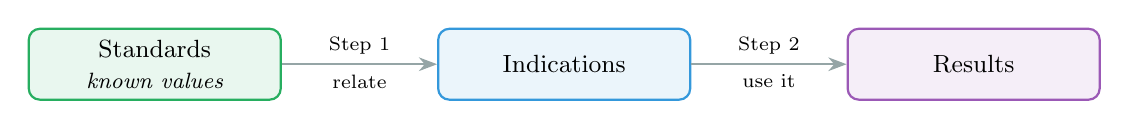
\begin{tikzpicture}
  \node[box=pass] (s) at (0,0) {Standards\\{\footnotesize\itshape known values}};
  \node[box=report] (i) at (5.2,0) {Indications};
  \node[box=state] (r) at (10.4,0) {Results};
  \draw[-{Stealth},thick,neutral] (s) -- node[above,font=\scriptsize,text=black]{Step 1} node[below,font=\scriptsize,text=black]{relate} (i);
  \draw[-{Stealth},thick,neutral] (i) -- node[above,font=\scriptsize,text=black]{Step 2} node[below,font=\scriptsize,text=black]{use it} (r);
\end{tikzpicture}
\end{center}

\vspace{0.1em}
{\small For the thermometer: read it against standards of known temperature, then use that relation to turn a length into a temperature. Step~1 alone is often mistaken for calibration, and so is adjusting the instrument.}

\vspace{0.3em}
{\small\textbf{Traceability} (VIM~2.41) is an unbroken, documented chain of calibrations back to a reference. It does not rule out mistakes, or an uncertainty too large for the purpose.}

\vspace{0.1em}
\begin{center}
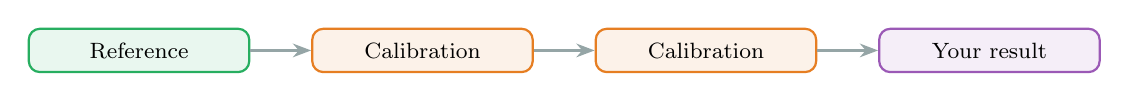
\begin{tikzpicture}
  \node[boxS=pass,minimum height=0.55cm] (a) at (0,0) {Reference};
  \node[boxS=bias,minimum height=0.55cm] (b) at (3.6,0) {Calibration};
  \node[boxS=bias,minimum height=0.55cm] (c) at (7.2,0) {Calibration};
  \node[boxS=state,minimum height=0.55cm] (d) at (10.8,0) {Your result};
  \draw[-{Stealth},thick,neutral] (a) -- (b);
  \draw[-{Stealth},thick,neutral] (b) -- (c);
  \draw[-{Stealth},thick,neutral] (c) -- (d);
\end{tikzpicture}
\end{center}
\end{frame}

\begin{frame}[label=uncertainty]{Uncertainty and its floor}
\textbf{Measurement uncertainty} (VIM~2.26) describes the spread of values that could be attributed to the measurand. It covers more than random scatter:

\vspace{0.4em}
\begin{center}
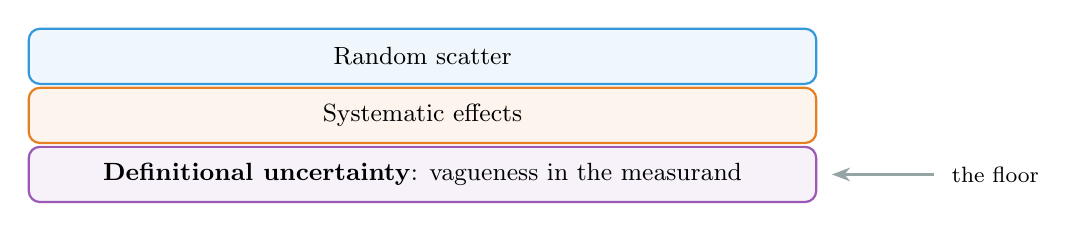
\begin{tikzpicture}
  \draw[panel=report] (0,1.5) rectangle (10,2.2);
  \node[font=\small] at (5,1.85) {Random scatter};
  \draw[panel=bias] (0,0.75) rectangle (10,1.45);
  \node[font=\small] at (5,1.1) {Systematic effects};
  \draw[panel=state] (0,0) rectangle (10,0.7);
  \node[font=\small] at (5,0.35) {\textbf{Definitional uncertainty}: vagueness in the measurand};
  \draw[-{Stealth},thick,neutral] (11.5,0.35) -- (10.2,0.35);
  \node[font=\footnotesize,anchor=west,text=black] at (11.6,0.35) {the floor};
\end{tikzpicture}
\end{center}

\vspace{0.4em}
Definitional uncertainty (VIM~2.27) is ``the practical minimum'' uncertainty achievable for a given measurand.

\vspace{0.2em}
{\small No instrument can be more precise than the measurand is defined. A better thermometer cannot fix a vague ``temperature of this water''.}
\end{frame}

\begin{frame}[label=sources]{Sources of uncertainty}
\begin{columns}[T]
\begin{column}{0.52\textwidth}
{\small The GUM lists ten sources (3.3.2). Five of them:}

\vspace{0.2em}
{\footnotesize\renewcommand{\arraystretch}{1.05}
\begin{tabular}{L{0.45cm}L{5.8cm}}
\toprule
(a) & Incomplete definition of the measurand \\
(c) & A sample that does not represent it \\
(d) & Incomplete knowledge of environmental effects \\
(i) & Approximations in the method \\
(j) & Variation in repeated observations \\
\bottomrule
\end{tabular}}

\vspace{0.3em}
{\small Repeating a measurement samples only (j). The GUM asks that all relevant quantities be varied as far as practicable (3.4.2).}
\end{column}
\begin{column}{0.47\textwidth}
\begin{center}
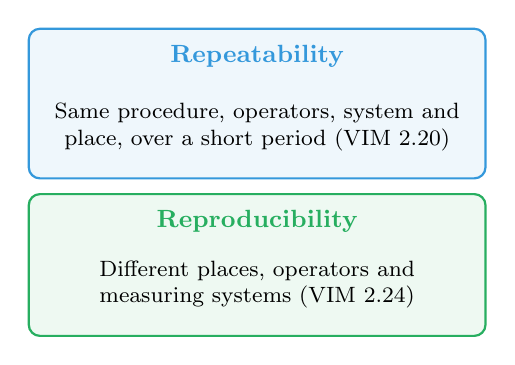
\begin{tikzpicture}
  \draw[panel=report] (0,2.0) rectangle (5.8,3.9);
  \node[font=\small\bfseries,text=report] at (2.9,3.55) {Repeatability};
  \node[font=\footnotesize,align=center,text width=5.4cm] at (2.9,2.65) {Same procedure, operators, system and place, over a short period (VIM~2.20)};
  \draw[panel=pass] (0,0) rectangle (5.8,1.8);
  \node[font=\small\bfseries,text=pass] at (2.9,1.45) {Reproducibility};
  \node[font=\footnotesize,align=center,text width=5.4cm] at (2.9,0.65) {Different places, operators and measuring systems (VIM~2.24)};
\end{tikzpicture}
\end{center}
\end{column}
\end{columns}
\end{frame}

\begin{frame}[label=compare]{Comparability and compatibility}
Two words that sound alike and ask different questions:

\vspace{0.5em}
\begin{center}
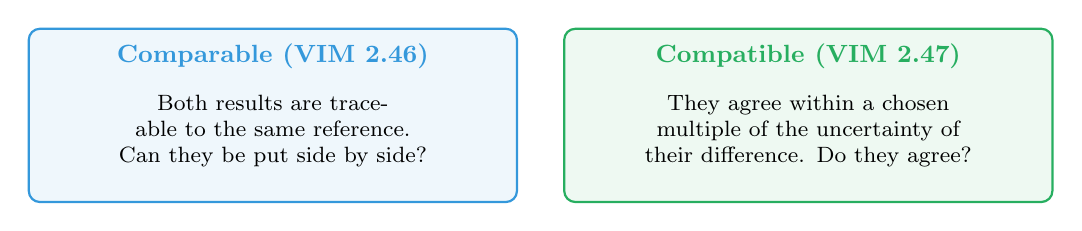
\begin{tikzpicture}
  \draw[panel=report] (0,0) rectangle (6.2,2.2);
  \node[font=\small\bfseries,text=report] at (3.1,1.85) {Comparable (VIM~2.46)};
  \node[font=\footnotesize,align=center,text width=5.7cm] at (3.1,0.9) {Both results are traceable to the same reference.\\Can they be put side by side?};
  \draw[panel=pass] (6.8,0) rectangle (13.0,2.2);
  \node[font=\small\bfseries,text=pass] at (9.9,1.85) {Compatible (VIM~2.47)};
  \node[font=\footnotesize,align=center,text width=5.7cm] at (9.9,0.9) {They agree within a chosen multiple of the uncertainty of their difference. Do they agree?};
\end{tikzpicture}
\end{center}

\vspace{0.6em}
The VIM uses compatibility to decide whether two results refer to \textbf{the same measurand} (2.47, Note~1).

\vspace{0.3em}
{\small Two thermometers traced to the same reference are comparable. Whether their readings are compatible is a separate question.}
\end{frame}

\begin{frame}[label=validation]{Validation for an intended use}
\textbf{Validation} (VIM~2.45) checks that specified requirements are adequate for an intended use. It is always relative to a use.

\vspace{0.5em}
\begin{center}
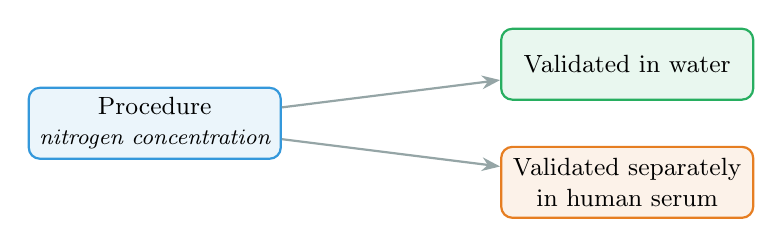
\begin{tikzpicture}
  \node[box=report] (p) at (0,0) {Procedure\\{\footnotesize\itshape nitrogen concentration}};
  \node[box=pass] (w) at (6,0.75) {Validated in water};
  \node[box=bias] (s) at (6,-0.75) {Validated separately\\in human serum};
  \draw[-{Stealth},thick,neutral] (p) -- (w);
  \draw[-{Stealth},thick,neutral] (p) -- (s);
\end{tikzpicture}
\end{center}

\vspace{0.5em}
The VIM's example: a procedure used for nitrogen in water may \emph{also} be validated for nitrogen in human serum. Validation in one setting does not carry over to another automatically.
\end{frame}

%% ============================================================
\partslide{part2}{Part 2\\[0.5em]{\large\mdseries The introspection experiment}}
%% ============================================================

\begin{frame}[label=injection]{Concept injection}
\href{https://arxiv.org/abs/2601.01828}{Lindsey (2025)} asks whether a language model notices a change to its own activations:

\vspace{0.3em}
\begin{enumerate}\setlength\itemsep{2pt}
  \item {\small Take a vector for a word such as \emph{bread}.}
  \item {\small Add it to the model's activations.}
  \item {\small Ask the model whether it detects an injected thought.}
\end{enumerate}

\vspace{0.2em}
\begin{center}
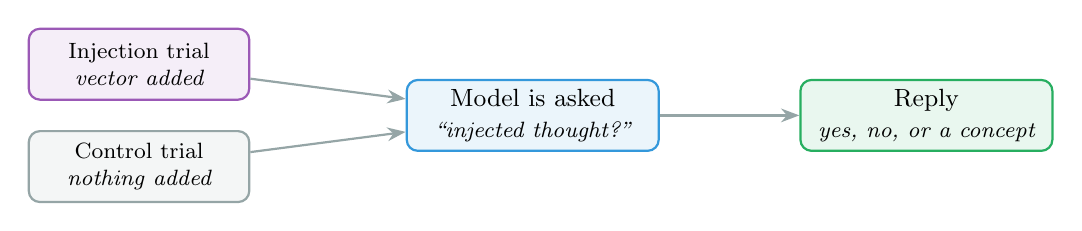
\begin{tikzpicture}
  \node[boxS=state] (a) at (0,0.65) {Injection trial\\{\footnotesize\itshape vector added}};
  \node[boxS=neutral] (b) at (0,-0.65) {Control trial\\{\footnotesize\itshape nothing added}};
  \node[box=report] (m) at (5,0) {Model is asked\\{\footnotesize\itshape ``injected thought?''}};
  \node[box=pass] (r) at (10,0) {Reply\\{\footnotesize\itshape yes, no, or a concept}};
  \draw[-{Stealth},thick,neutral] (a) -- (m);
  \draw[-{Stealth},thick,neutral] (b) -- (m);
  \draw[-{Stealth},thick,neutral] (m) -- (r);
\end{tikzpicture}
\end{center}

\vspace{0.2em}
{\small The next slides put this experiment through the vocabulary of Part~1.}
\end{frame}

\begin{frame}[label=mapping]{The experiment in the vocabulary}
\begin{center}
{\footnotesize\renewcommand{\arraystretch}{1.1}
\begin{tabular}{L{2.4cm}L{3.6cm}L{6.4cm}}
\toprule
\textbf{Term} & \textbf{Thermometer} & \textbf{Concept injection} \\
\midrule
Measurand & Temperature of the water & ``Introspective access'', which admits several readings \\
Realized quantity & What is actually measured & The injected state, an approximation of the states the claim is about \\
Indication & A length of mercury & The reply: a string, a yes or no, a number, a choice \\
Result & A temperature & The claim that the model has access to a state \\
Blank indication & Quantity supposed absent & Control trials without injection \\
\bottomrule
\end{tabular}}
\end{center}

\vspace{0.4em}
{\small Lindsey reports no false positives in 100 control trials. The vagueness of ``introspective access'' is definitional uncertainty, and under the VIM it belongs inside the error bar.}
\end{frame}

\begin{frame}[label=twosenses]{Two senses of calibration}
The introspection literature often uses ``calibration'' in a different sense from the VIM.

\vspace{0.5em}
\begin{center}
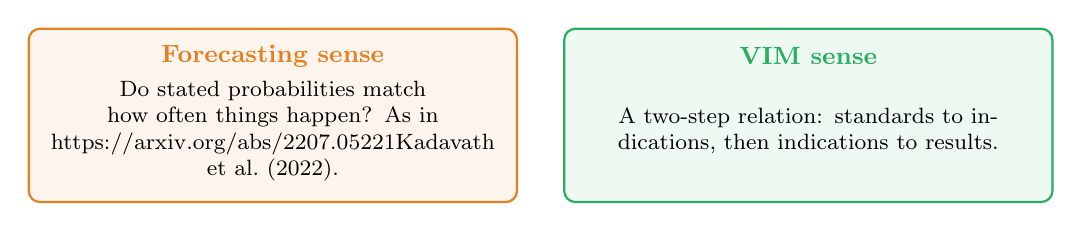
\begin{tikzpicture}
  \draw[panel=bias] (0,0) rectangle (6.2,2.2);
  \node[font=\small\bfseries,text=bias] at (3.1,1.85) {Forecasting sense};
  \node[font=\footnotesize,align=center,text width=5.7cm] at (3.1,0.9) {Do stated probabilities match how often things happen? As in \href{https://arxiv.org/abs/2207.05221}{Kadavath et al.\ (2022)}.};
  \draw[panel=pass] (6.8,0) rectangle (13.0,2.2);
  \node[font=\small\bfseries,text=pass] at (9.9,1.85) {VIM sense};
  \node[font=\footnotesize,align=center,text width=5.7cm] at (9.9,0.9) {A two-step relation: standards to indications, then indications to results.};
\end{tikzpicture}
\end{center}

\vspace{0.5em}
The measurement card uses the VIM sense. A model can be calibrated in the first sense without its reports being tied to any reference in the second.

\vspace{0.3em}
{\small The \href{https://measuring-self-reports.github.io/measuring-self-reports/foundations/signal-detection/}{signal detection page} separates the senses further.}
\end{frame}

\begin{frame}[label=llmunc]{Uncertainty in an injection experiment}
The influence quantities of an injection measurement:

\vspace{0.3em}
\begin{center}
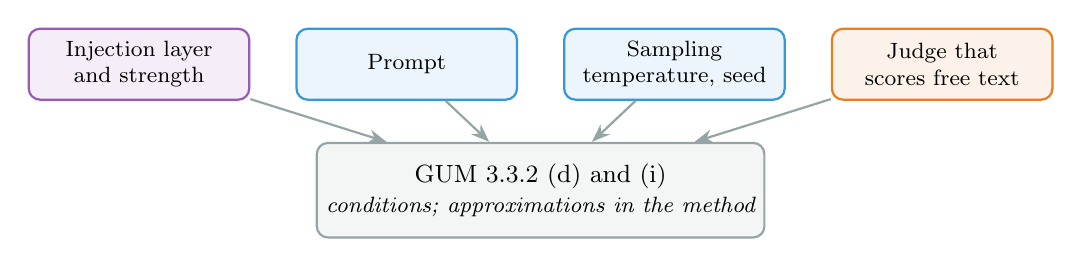
\begin{tikzpicture}
  \node[boxS=state] (a) at (0,0) {Injection layer\\and strength};
  \node[boxS=report] (b) at (3.4,0) {Prompt};
  \node[boxS=report] (c) at (6.8,0) {Sampling\\temperature, seed};
  \node[boxS=bias] (d) at (10.2,0) {Judge that\\scores free text};
  \node[boxL=neutral] (g) at (5.1,-1.6) {GUM 3.3.2 (d) and (i)\\{\footnotesize\itshape conditions; approximations in the method}};
  \draw[-{Stealth},thick,neutral] (a) -- (g);
  \draw[-{Stealth},thick,neutral] (b) -- (g);
  \draw[-{Stealth},thick,neutral] (c) -- (g);
  \draw[-{Stealth},thick,neutral] (d) -- (g);
\end{tikzpicture}
\end{center}

\vspace{0.3em}
The GUM asks that these be varied (3.4.2). Resampling at one prompt and one judge samples only source (j).

\vspace{0.2em}
{\small Changing the judge or the prompt is a change of measuring system: a \textbf{reproducibility} condition (VIM~2.24).}
\end{frame}

\begin{frame}[label=limitsmet]{Where the analogy stops: metrology}
\begin{itemize}\setlength\itemsep{8pt}
  \item {\small \textbf{Nominal outcomes.} Measurement does not apply to nominal properties (VIM~2.1, Note~1). Many introspection outcomes are nominal, such as which concept was injected, so the vocabulary applies to them only by analogy.}
  \item {\small \textbf{No calibration hierarchy.} No reference procedure, standard or unit anchors a report of a model's internal state. Traceability has no chain to run along, and comparability in the VIM sense is unavailable. The card asks what a paper used in place of a reference, and whether the model under test produced it.}
  \item {\small \textbf{No model of the disturbance.} The voltmeter correction assumes a model of the disturbance. In self-report the instrument and the object are the same network, and no such model is available.}
\end{itemize}
\end{frame}

%% ============================================================
\partslide{part3}{Part 3\\[0.5em]{\large\mdseries Robustness and convergence}}
%% ============================================================

\begin{frame}[label=wimsatt]{Robustness analysis}
Agreement among independent procedures is evidence that a result is real, not an artifact of one procedure. \href{https://link.springer.com/chapter/10.1007/978-94-007-2759-5_2}{Wimsatt (1981)} gives four steps:

\vspace{0.4em}
\begin{center}
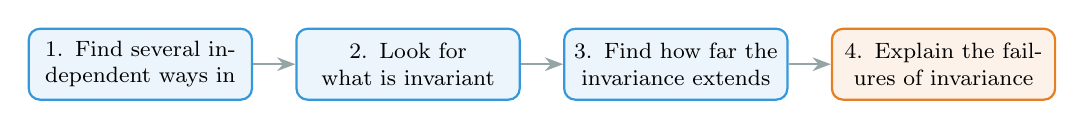
\begin{tikzpicture}
  \node[boxS=report,text width=2.6cm] (a) at (0,0) {1. Find several independent ways in};
  \node[boxS=report,text width=2.6cm] (b) at (3.4,0) {2. Look for what is invariant};
  \node[boxS=report,text width=2.6cm] (c) at (6.8,0) {3. Find how far the invariance extends};
  \node[boxS=bias,text width=2.6cm] (d) at (10.2,0) {4. Explain the failures of invariance};
  \draw[-{Stealth},thick,neutral] (a) -- (b);
  \draw[-{Stealth},thick,neutral] (b) -- (c);
  \draw[-{Stealth},thick,neutral] (c) -- (d);
\end{tikzpicture}
\end{center}

\vspace{0.4em}
{\small Step~4 treats failures of invariance as information. Wimsatt also says why one route is weak: a quantity reached only one way cannot be tested independently.}

\vspace{0.3em}
{\small Evidence for introspection in a language model often takes this form: a self-report matches a probe, an intervention or a second prompt format.}
\end{frame}

\begin{frame}[label=illusory]{Illusory robustness}
When procedures are presumed independent and are not, the result is \textbf{\textcolor{fail}{illusory robustness}}. Wimsatt calls it the most striking way robustness analysis fails.

\vspace{0.3em}
\begin{center}
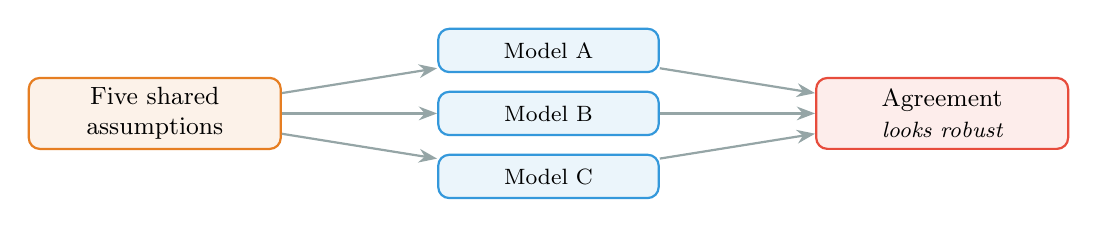
\begin{tikzpicture}
  \node[box=bias] (s) at (0,0) {Five shared\\assumptions};
  \node[boxS=report,minimum height=0.55cm] (m1) at (5,0.8) {Model A};
  \node[boxS=report,minimum height=0.55cm] (m2) at (5,0) {Model B};
  \node[boxS=report,minimum height=0.55cm] (m3) at (5,-0.8) {Model C};
  \node[box=fail] (a) at (10,0) {Agreement\\{\footnotesize\itshape looks robust}};
  \draw[-{Stealth},thick,neutral] (s) -- (m1);
  \draw[-{Stealth},thick,neutral] (s) -- (m2);
  \draw[-{Stealth},thick,neutral] (s) -- (m3);
  \draw[-{Stealth},thick,neutral] (m1) -- (a);
  \draw[-{Stealth},thick,neutral] (m2) -- (a);
  \draw[-{Stealth},thick,neutral] (m3) -- (a);
\end{tikzpicture}
\end{center}

\vspace{0.2em}
{\small His case: group-selection models that agreed because they shared five assumptions, a form of method bias. Such failures are hard to detect. Tal (\href{https://plato.stanford.edu/entries/measurement-science/}{SEP~\S8.3}) states the measurement version: inaccurate measurements can share a bias, so their errors do not cancel when averaged.}
\end{frame}

\begin{frame}[label=cf]{Independence of methods}
\href{https://www.ovid.com/journals/plbul/fulltext/00006823-195903000-00001~convergent-and-discriminant-validation-by-the}{Campbell and Fiske (1959)}, Wimsatt's source for method bias, treat independence as a matter of degree:

\vspace{0.3em}
\begin{center}
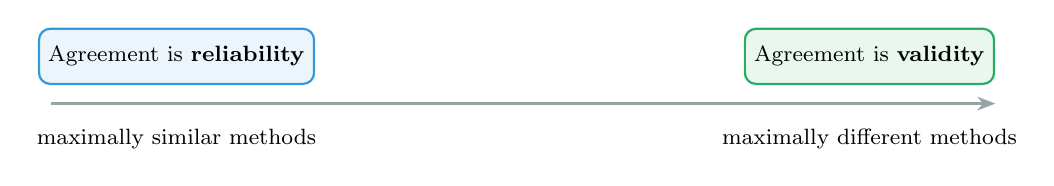
\begin{tikzpicture}
  \draw[-{Stealth},thick,neutral] (0,0) -- (12,0);
  \node[font=\footnotesize,align=center,text=black] at (1.6,-0.45) {maximally similar methods};
  \node[font=\footnotesize,align=center,text=black] at (10.4,-0.45) {maximally different methods};
  \node[boxS=report,minimum height=0.7cm] at (1.6,0.6) {Agreement is \textbf{reliability}};
  \node[boxS=pass,minimum height=0.7cm] at (10.4,0.6) {Agreement is \textbf{validity}};
\end{tikzpicture}
\end{center}

\vspace{0.2em}
{\small Shared method shows up only when \textbf{several traits} are measured by \textbf{several methods}; otherwise a high correlation could reflect the trait or the method. The check: a measure should agree more with a different method on the same trait than with the same method on a different trait. The \href{https://measuring-self-reports.github.io/measuring-self-reports/foundations/psychometrics/}{psychometrics page} covers their matrix.}
\end{frame}

\begin{frame}[label=perrin]{Perrin's convergence and Hudson's reading}
\small Jean Perrin determined Avogadro's number from more than a dozen phenomena, such as Brownian motion and radioactivity, and argued that their agreement made molecules nearly certain. \href{https://academic.oup.com/book/9863}{Hudson (2013)} reads the reasoning differently.

\vspace{0.1em}
\begin{columns}[T]
\begin{column}{0.48\textwidth}
\begin{center}
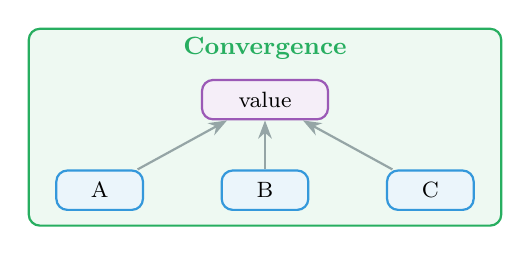
\begin{tikzpicture}
  \draw[panel=pass] (-0.3,-0.3) rectangle (5.7,2.2);
  \node[font=\small\bfseries,text=pass] at (2.7,1.95) {Convergence};
  \node[boxS=report,minimum width=1.1cm,minimum height=0.5cm] (a) at (0.6,0.15) {A};
  \node[boxS=report,minimum width=1.1cm,minimum height=0.5cm] (b) at (2.7,0.15) {B};
  \node[boxS=report,minimum width=1.1cm,minimum height=0.5cm] (c) at (4.8,0.15) {C};
  \node[boxS=state,minimum width=1.6cm,minimum height=0.5cm] (n) at (2.7,1.3) {value};
  \draw[-{Stealth},thick,neutral] (a) -- (n);
  \draw[-{Stealth},thick,neutral] (b) -- (n);
  \draw[-{Stealth},thick,neutral] (c) -- (n);
\end{tikzpicture}
\end{center}
{\footnotesize Methods agree as equals, and the agreement supports all of them at once.}
\end{column}
\begin{column}{0.48\textwidth}
\begin{center}
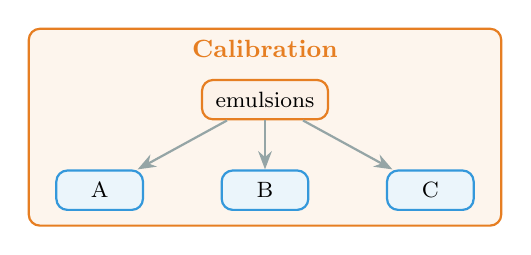
\begin{tikzpicture}
  \draw[panel=bias] (-0.3,-0.3) rectangle (5.7,2.2);
  \node[font=\small\bfseries,text=bias] at (2.7,1.95) {Calibration};
  \node[boxS=bias,minimum width=1.6cm,minimum height=0.5cm] (p) at (2.7,1.3) {emulsions};
  \node[boxS=report,minimum width=1.1cm,minimum height=0.5cm] (a) at (0.6,0.15) {A};
  \node[boxS=report,minimum width=1.1cm,minimum height=0.5cm] (b) at (2.7,0.15) {B};
  \node[boxS=report,minimum width=1.1cm,minimum height=0.5cm] (c) at (4.8,0.15) {C};
  \draw[-{Stealth},thick,neutral] (p) -- (a);
  \draw[-{Stealth},thick,neutral] (p) -- (b);
  \draw[-{Stealth},thick,neutral] (p) -- (c);
\end{tikzpicture}
\end{center}
{\footnotesize Hudson's reading: Perrin's emulsion experiments were the standard. The rest are supported only as far as it is trusted.}
\end{column}
\end{columns}
\end{frame}

\begin{frame}[label=islands]{Coherence and islands}
\href{https://philpapers.org/rec/TALCMT}{Tal (2017)} treats calibration as a test of invariance across instruments and circumstances. Agreement is not enough: each uncertainty must come from an adequate model of the process.

\vspace{0.4em}
\begin{center}
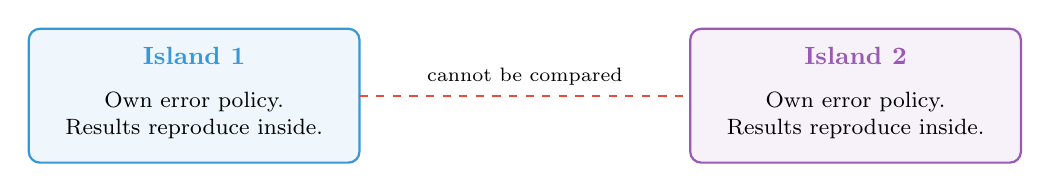
\begin{tikzpicture}
  \draw[panel=report] (0,0) rectangle (4.2,1.7);
  \node[font=\small\bfseries,text=report] at (2.1,1.35) {Island 1};
  \node[font=\footnotesize,align=center,text width=3.8cm] at (2.1,0.6) {Own error policy.\\Results reproduce inside.};
  \draw[panel=state] (8.4,0) rectangle (12.6,1.7);
  \node[font=\small\bfseries,text=state] at (10.5,1.35) {Island 2};
  \node[font=\footnotesize,align=center,text width=3.8cm] at (10.5,0.6) {Own error policy.\\Results reproduce inside.};
  \draw[dashed,fail,thick] (4.2,0.85) -- node[above,font=\scriptsize,text=black]{cannot be compared} (8.4,0.85);
\end{tikzpicture}
\end{center}

\vspace{0.3em}
{\small The same indications can be made coherent in more than one way, so a network of instruments can split into islands. Tal's example: the 1990 conventional values for electrical standards, which raised internal consistency and created an island. The remedy is standards that impose one error policy on the network.}
\end{frame}

%% ============================================================
\partslide{part4}{Part 4\\[0.5em]{\large\mdseries Robustness in AI introspection}}
%% ============================================================

\begin{frame}[label=shared]{A report and a probe on the same activations}
\begin{columns}[c]
\begin{column}{0.47\textwidth}
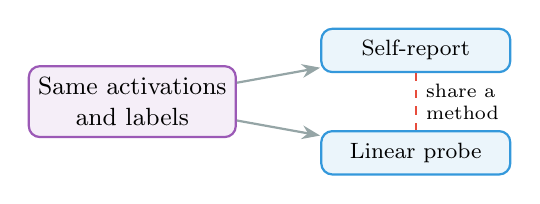
\begin{tikzpicture}
  \node[box=state,minimum width=2.6cm] (x) at (0,0) {Same activations\\and labels};
  \node[boxS=report,minimum height=0.55cm,minimum width=2.4cm] (r) at (3.6,0.65) {Self-report};
  \node[boxS=report,minimum height=0.55cm,minimum width=2.4cm] (p) at (3.6,-0.65) {Linear probe};
  \draw[-{Stealth},thick,neutral] (x) -- (r);
  \draw[-{Stealth},thick,neutral] (x) -- (p);
  \draw[dashed,fail,thick] (r) -- node[right,font=\scriptsize,text=black,align=left]{share a\\method} (p);
\end{tikzpicture}
\end{column}
\begin{column}{0.49\textwidth}
{\small A report and a probe trained on the same activations and labels share part of their method, as do two prompts scored by one judge. Their agreement is exposed to illusory robustness.}
\end{column}
\end{columns}

\vspace{0.3em}
{\small \textbf{Campbell and Fiske's test}: a report and a probe on one state should agree more than readings of two different states taken with the same prompt, layer or judge.}

\begin{center}
{\footnotesize\renewcommand{\arraystretch}{1.05}
\begin{tabular}{lll}
\toprule
& \textbf{Same state} & \textbf{Different states} \\
\midrule
\textbf{Different procedures} & should agree \textbf{more}\ldots & \\
\textbf{Same prompt, layer or judge} & & \ldots than these \\
\bottomrule
\end{tabular}}
\end{center}
\end{frame}

\begin{frame}[label=structure]{Convergence, calibration and islands}
Following Hudson, an introspection paper can have either of Perrin's structures:

\vspace{0.3em}
\begin{center}
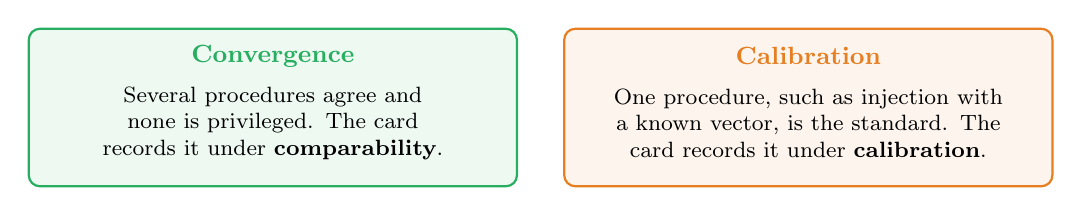
\begin{tikzpicture}
  \draw[panel=pass] (0,0) rectangle (6.2,2.0);
  \node[font=\small\bfseries,text=pass] at (3.1,1.65) {Convergence};
  \node[font=\footnotesize,align=center,text width=5.7cm] at (3.1,0.8) {Several procedures agree and none is privileged. The card records it under \textbf{comparability}.};
  \draw[panel=bias] (6.8,0) rectangle (13.0,2.0);
  \node[font=\small\bfseries,text=bias] at (9.9,1.65) {Calibration};
  \node[font=\footnotesize,align=center,text width=5.7cm] at (9.9,0.8) {One procedure, such as injection with a known vector, is the standard. The card records it under \textbf{calibration}.};
\end{tikzpicture}
\end{center}

\vspace{0.4em}
{\small\textbf{Islands.} When each group scores introspection with its own prompts, judges and thresholds, results can reproduce within each setup and fail to compare across setups.}
\end{frame}

\begin{frame}[label=limitsrob]{Where the analogy stops: robustness}
\begin{itemize}\setlength\itemsep{10pt}
  \item {\small \textbf{Same substrate.} Perrin's methods rested on different physical phenomena with separate theories. Every procedure for reading a language model's internal state acts on the same network, often at the same layers. Independence has to be argued case by case.}
  \item {\small \textbf{No standards body.} Tal's remedy for islands is institutional. No body or standard exists for the internal states of models.}
\end{itemize}
\end{frame}

\begin{frame}[label=summary]{Summary}
\begin{center}
{\footnotesize\renewcommand{\arraystretch}{1.0}
\begin{tabular}{L{3.6cm}L{6.4cm}L{2.6cm}}
\toprule
\textbf{Idea} & \textbf{Question for an introspection experiment} & \textbf{Card stage} \\
\midrule
Definitional uncertainty & Which reading of ``introspective access''? & Measurand \\
Blank indication & What do the control trials show? & Instrument \\
VIM calibration & What stands in for a reference? Did the model make it? & Calibration \\
Sources of uncertainty & Were layer, prompt, seed and judge varied? & Uncertainty \\
Compatibility & Do results agree within their uncertainty? & Comparability \\
Validation & Was the procedure validated for this use? & Validity conditions \\
Illusory robustness & What do the agreeing procedures share? & Comparability \\
Hudson on Perrin & Convergence among equals, or one standard? & Calibration \\
Islands & Do results compare across setups? & Comparability \\
\bottomrule
\end{tabular}
}
\end{center}
\end{frame}

\begin{frame}[label=reading]{Reading}
\footnotesize
\begin{itemize}\setlength\itemsep{1pt}
  \item \href{https://www.bipm.org/documents/20126/2071204/JCGM_200_2012.pdf}{International Vocabulary of Metrology (VIM)}, JCGM 200:2012: the defined terms.
  \item \href{https://www.bipm.org/documents/20126/2071204/JCGM_100_2008_E.pdf}{Guide to the Expression of Uncertainty in Measurement (GUM)}, JCGM 100:2008.
  \item \href{https://link.springer.com/chapter/10.1007/978-94-007-2759-5_2}{Wimsatt, Robustness, reliability, and overdetermination} (1981): illusory robustness.
  \item \href{https://www.ovid.com/journals/plbul/fulltext/00006823-195903000-00001~convergent-and-discriminant-validation-by-the}{Campbell and Fiske, Convergent and discriminant validation} (1959): independence of methods.
  \item \href{https://academic.oup.com/book/9863}{Hudson, Seeing Things} (2013), ch.~4: Perrin's reasoning as calibration.
  \item \href{https://philpapers.org/rec/TALCMT}{Tal, Calibration: Modelling the measurement process} (2017): coherence and islands.
  \item \href{https://plato.stanford.edu/entries/measurement-science/}{Tal, Measurement in Science} (SEP), \S8.3: common bias.
  \item \href{https://arxiv.org/abs/2601.01828}{Lindsey, Emergent introspective awareness in large language models} (2025).
  \item \href{https://arxiv.org/abs/2207.05221}{Kadavath et al., Language models (mostly) know what they know} (2022).
\end{itemize}
\end{frame}

\end{document}
